\documentclass[11pt]{article}
\usepackage[hmargin=1in,vmargin=1in]{geometry}
\usepackage[table]{xcolor} 
\usepackage{amsmath,amssymb,amsfonts,url,sectsty,tcolorbox,framed}
\usepackage{hyperref}
\usepackage{listings}
\usepackage{booktabs}
\usepackage{array}
\usepackage{multirow}
\usepackage{graphicx}
\usepackage{tikz}
\usetikzlibrary{arrows.meta, positioning, shapes.geometric, fit, backgrounds, calc}
\usepackage{pgfplots}
\pgfplotsset{compat=1.18}
\usepackage{fancyhdr}
\usepackage{fontawesome5}
\usepackage{enumitem}

% ──────────────────────────────────────────────────────
% COLOR PALETTE
% ──────────────────────────────────────────────────────
\definecolor{lightblue}{rgb}{0.8,0.9,1}
\definecolor{codebg}{RGB}{250, 250, 250}
\definecolor{codeframe}{RGB}{200, 200, 200}
\definecolor{tableheader}{RGB}{41, 128, 185}
\definecolor{rowalt}{RGB}{235, 245, 251}
\definecolor{accentblue}{RGB}{52, 152, 219}
\definecolor{accentgreen}{RGB}{39, 174, 96}
\definecolor{accentorange}{RGB}{230, 126, 34}
\definecolor{accentred}{RGB}{231, 76, 60}
\definecolor{accentpurple}{RGB}{142, 68, 173}
\definecolor{darkbg}{RGB}{30, 30, 30}
\definecolor{codekw}{RGB}{86, 156, 214}
\definecolor{codecomment}{RGB}{106, 153, 85}
\definecolor{codestring}{RGB}{206, 145, 120}
\definecolor{codenumber}{RGB}{181, 206, 168}
\definecolor{codetype}{RGB}{78, 201, 176}
\definecolor{sectioncolor}{RGB}{41, 128, 185}

% ──────────────────────────────────────────────────────
% SECTION STYLING
% ──────────────────────────────────────────────────────
\sectionfont{\color{sectioncolor}}
\subsectionfont{\color{sectioncolor!80!black}}
\subsubsectionfont{\color{sectioncolor!60!black}}

% ──────────────────────────────────────────────────────
% HYPERLINK STYLING
% ──────────────────────────────────────────────────────
\hypersetup{
    colorlinks=true,
    linkcolor=sectioncolor,
    urlcolor=accentblue,
    citecolor=accentgreen,
    pdfborder={0 0 0}
}

% ──────────────────────────────────────────────────────
% HEADER / FOOTER
% ──────────────────────────────────────────────────────
\pagestyle{fancy}
\fancyhf{}
\fancyhead[L]{\small\color{gray}\textsc{Lab 4: Parallel BOGO Sort}}
\fancyhead[R]{\small\color{gray}\textsc{CS302 -- DPC}}
\fancyfoot[C]{\small\color{gray}\thepage}
\renewcommand{\headrulewidth}{0.4pt}
\renewcommand{\footrulewidth}{0pt}
\fancypagestyle{plain}{\fancyhf{}\fancyfoot[C]{\small\color{gray}\thepage}\renewcommand{\headrulewidth}{0pt}}

% ──────────────────────────────────────────────────────
% CODE STYLE CONFIGURATION (VS Code Dark+ inspired)
% ──────────────────────────────────────────────────────
\lstset{
    backgroundcolor=\color{darkbg},
    basicstyle=\ttfamily\small\color{white},
    breaklines=true,
    breakatwhitespace=false,
    commentstyle=\color{codecomment}\itshape,
    keywordstyle=\color{codekw}\bfseries,
    stringstyle=\color{codestring},
    numberstyle=\tiny\color{gray},
    numbers=left,
    numbersep=8pt,
    stepnumber=1,
    frame=none,
    showstringspaces=false,
    language=C++,
    tabsize=4,
    columns=fullflexible,
    keepspaces=true,
    xleftmargin=10pt,
    morekeywords={volatile, mt19937, uniform_int_distribution, vector, memcpy, shuffle, omp_set_num_threads, omp_get_thread_num, omp_get_wtime},
    emphstyle={\color{codetype}},
    emph={int, bool, long, double, void, const, ParallelResult},
    literate=
        {0}{{\textcolor{codenumber}{0}}}1
        {1}{{\textcolor{codenumber}{1}}}1
        {2}{{\textcolor{codenumber}{2}}}1
        {3}{{\textcolor{codenumber}{3}}}1
        {4}{{\textcolor{codenumber}{4}}}1
        {5}{{\textcolor{codenumber}{5}}}1
        {6}{{\textcolor{codenumber}{6}}}1
        {7}{{\textcolor{codenumber}{7}}}1
        {8}{{\textcolor{codenumber}{8}}}1
        {9}{{\textcolor{codenumber}{9}}}1
        {\#pragma}{{\textcolor{accentpurple}{\#pragma}}}7
}

% ──────────────────────────────────────────────────────
% BOX DEFINITIONS
% ──────────────────────────────────────────────────────
\tcbuselibrary{breakable, skins, listings}

% Code block box (dark themed)
\newtcolorbox{codebox}[1][]{%
    enhanced,
    breakable,
    colback=darkbg,
    colframe=darkbg!60!black,
    title={\faCode\ \ #1},
    fonttitle=\bfseries\sffamily\small\color{white},
    coltitle=white,
    arc=4pt,
    boxrule=0.8pt,
    top=2pt,
    bottom=2pt,
    left=0pt,
    right=4pt,
    before skip=10pt,
    after skip=10pt,
    shadow={1mm}{-1mm}{0mm}{black!30},
    attach boxed title to top left={xshift=10pt, yshift=-\tcboxedtitleheight/2},
    boxed title style={colback=accentblue, arc=3pt, boxrule=0pt, left=6pt, right=6pt}
}

% Explanation / concept box
\newtcolorbox{shadedbox}[1][]{%
    enhanced,
    breakable,
    colback=lightblue!15,
    colframe=accentblue,
    title={\faLightbulb[regular]\ \ #1},
    fonttitle=\bfseries\sffamily,
    coltitle=white,
    arc=4pt,
    boxrule=0.8pt,
    before skip=10pt,
    after skip=10pt,
    shadow={1mm}{-1mm}{0mm}{accentblue!20},
    attach boxed title to top left={xshift=10pt, yshift=-\tcboxedtitleheight/2},
    boxed title style={colback=accentblue, arc=3pt, boxrule=0pt, left=6pt, right=6pt}
}

% Terminal output box
\newtcolorbox{terminalbox}[1]{%
    enhanced,
    breakable,
    colback=darkbg,
    colframe=darkbg!40!black,
    colupper=white,
    title={\faTerminal\ \ #1},
    fonttitle=\bfseries\ttfamily\small\color{white},
    coltitle=white,
    arc=4pt,
    boxrule=0.8pt,
    before skip=10pt,
    after skip=10pt,
    shadow={1mm}{-1mm}{0mm}{black!30},
    attach boxed title to top left={xshift=10pt, yshift=-\tcboxedtitleheight/2},
    boxed title style={colback=accentgreen!80!black, arc=3pt, boxrule=0pt, left=6pt, right=6pt}
}

% Warning / important box
\newtcolorbox{warningbox}[1][]{%
    enhanced,
    breakable,
    colback=accentorange!8,
    colframe=accentorange,
    title={\faExclamationTriangle\ \ #1},
    fonttitle=\bfseries\sffamily,
    coltitle=white,
    arc=4pt,
    boxrule=0.8pt,
    before skip=10pt,
    after skip=10pt,
    attach boxed title to top left={xshift=10pt, yshift=-\tcboxedtitleheight/2},
    boxed title style={colback=accentorange, arc=3pt, boxrule=0pt, left=6pt, right=6pt}
}

% Style for the code within the terminal
\lstdefinestyle{terminalstyle}{
    basicstyle=\ttfamily\small\color{white},
    breaklines=true,
    language=bash,
    numbers=none,
    literate={>}{{\textcolor{accentgreen}{>}}}1,
    columns=fullflexible,
    keepspaces=true,
    frame=none,
    backgroundcolor=\color{darkbg},
    xleftmargin=8pt
}

% Style for inline code in bash/terminal
\lstdefinestyle{bashstyle}{
    language=bash,
    basicstyle=\ttfamily\small\color{white},
    backgroundcolor=\color{darkbg},
    keywordstyle=\color{accentgreen}\bfseries,
    commentstyle=\color{gray}\itshape,
    numbers=none,
    frame=none,
    xleftmargin=8pt,
    breaklines=true,
    columns=fullflexible,
    keepspaces=true
}

\begin{document}

% ══════════════════════════════════════════════════════
% TITLE PAGE
% ══════════════════════════════════════════════════════
\thispagestyle{empty}
\begin{center}
\vspace*{1cm}

{\color{sectioncolor}\rule{\textwidth}{2pt}}
\vspace{0.3cm}

{\Huge\bfseries\sffamily\color{sectioncolor} Parallel BOGO Sort}

\vspace{0.15cm}
{\Large\sffamily\color{gray} Performance Study using OpenMP}

\vspace{0.3cm}
{\color{sectioncolor}\rule{\textwidth}{2pt}}

\vspace{1.2cm}

{\large\sffamily\color{sectioncolor} [CS302] Distributed and Parallel Computing}

\vspace{1.5cm}

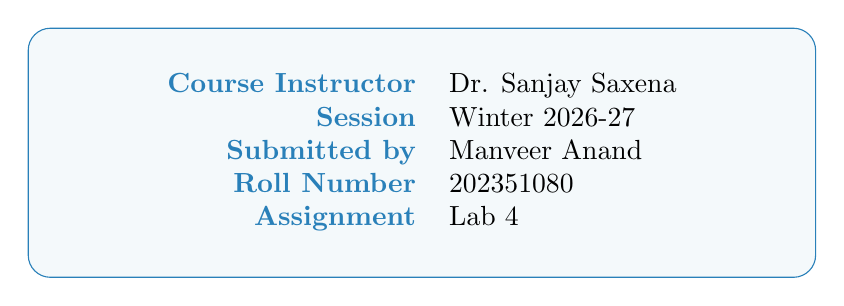
\begin{tikzpicture}
\node[draw=sectioncolor, fill=sectioncolor!5, rounded corners=8pt, inner sep=15pt, minimum width=10cm] {
    \begin{tabular}{r @{\hspace{12pt}} l}
    \textbf{\color{sectioncolor}Course Instructor} & Dr. Sanjay Saxena \\
    \textbf{\color{sectioncolor}Session} & Winter 2026-27 \\
    \textbf{\color{sectioncolor}Submitted by} & Manveer Anand \\
    \textbf{\color{sectioncolor}Roll Number} & 202351080 \\
    \textbf{\color{sectioncolor}Assignment} & Lab 4 \\
    \end{tabular}
};
\end{tikzpicture}

\vspace{1.5cm}

{\color{gray}\small OpenMP Concepts: \texttt{parallel} $\cdot$ \texttt{critical} $\cdot$ \texttt{atomic} $\cdot$ \texttt{barrier} $\cdot$ \texttt{thread control}}

\vfill
{\color{gray}\small\today}
\end{center}
\newpage

\tableofcontents
\newpage 

\section{Introduction}
This assignment implements BOGO Sort in both sequential and parallel forms using OpenMP. BOGO Sort is a highly inefficient sorting algorithm based on randomness---it repeatedly shuffles the array until it becomes sorted. Although impractical for real-world sorting, it serves as an excellent case study for \textbf{parallel trial-based computation}, where multiple threads attempt the same task simultaneously and the first successful result terminates the process.

\subsection{Key Requirements}
\begin{enumerate}
    \item Implement sequential BOGO Sort as a performance baseline.
    \item Implement parallel BOGO Sort using OpenMP with 2, 4, and 8 threads.
    \item Each thread independently shuffles its own copy of the array.
    \item The first thread to find a sorted permutation signals all others to stop.
    \item Compare execution times, shuffle counts, and compute speedup.
\end{enumerate}

\subsection{BOGO Sort Algorithm}
Given an array $A$ of size $N$:
\begin{enumerate}
    \item Check if $A$ is sorted.
    \item If sorted, stop.
    \item Otherwise, shuffle $A$ randomly and repeat.
\end{enumerate}

The expected number of shuffles for $N$ unique elements is $N!$, making the average time complexity $O(N \times N!)$.

\subsection{Input Specification}
\begin{itemize}
    \item Array sizes tested: $N = 10$ and $N = 12$
    \item Values: Unique integers randomly selected from range $[1, 50]$
    \item Generation: Fisher-Yates shuffle on pool of values 1--50, pick first $N$
\end{itemize}

\newpage

\section{Architecture Design}

\subsection{Parallelization Strategy}

The parallel approach exploits the probabilistic nature of BOGO Sort. Since each shuffle is an independent random trial, multiple threads can attempt different shuffles concurrently. The first thread to stumble upon the sorted permutation wins.

\begin{shadedbox}[Parallel BOGO Sort Architecture]
\textbf{1. Thread Independence} \\
Each thread receives its own \textit{copy} of the original array and its own random number generator (seeded uniquely per thread). Threads shuffle independently without any shared data access on the array itself.

\vspace{6pt}
\textbf{2. Shared Termination Flag} (\texttt{volatile int found = 0}) \\
A shared atomic flag acts as the stop signal. All threads check this flag before each shuffle iteration. When a thread finds a sorted permutation, it sets \texttt{found = 1} inside a \texttt{\#pragma omp critical} block.

\vspace{6pt}
\textbf{3. Result Collection} \\
The winning thread copies its sorted array into a shared result buffer (protected by the critical section). After the parallel region, each thread's local shuffle count is accumulated using \texttt{\#pragma omp atomic}.
\end{shadedbox}

\subsection{OpenMP Constructs Used}

\begin{center}
\sffamily\small
\begin{tabular}{@{}llp{7.5cm}@{}}
\toprule
\rowcolor{tableheader}
\textcolor{white}{\textbf{Construct}} & \textcolor{white}{\textbf{Directive}} & \textcolor{white}{\textbf{Purpose}} \\
\midrule
\rowcolor{rowalt}
Parallel Region & \texttt{\#pragma omp parallel} & Spawns $T$ threads, each running BOGO Sort independently \\
Critical Section & \texttt{\#pragma omp critical} & Protects the shared result buffer and \texttt{found} flag from race conditions \\
\rowcolor{rowalt}
Atomic Operation & \texttt{\#pragma omp atomic} & Safely accumulates total shuffle count from all threads \\
Thread Control & \texttt{omp\_set\_num\_threads(T)} & Sets the number of threads for each experiment \\
\rowcolor{rowalt}
Thread ID & \texttt{omp\_get\_thread\_num()} & Identifies which thread found the solution \\
Wall Clock & \texttt{omp\_get\_wtime()} & High-resolution timing for performance measurement \\
\bottomrule
\end{tabular}
\end{center}

\subsection{Thread Execution Flow}

\begin{center}
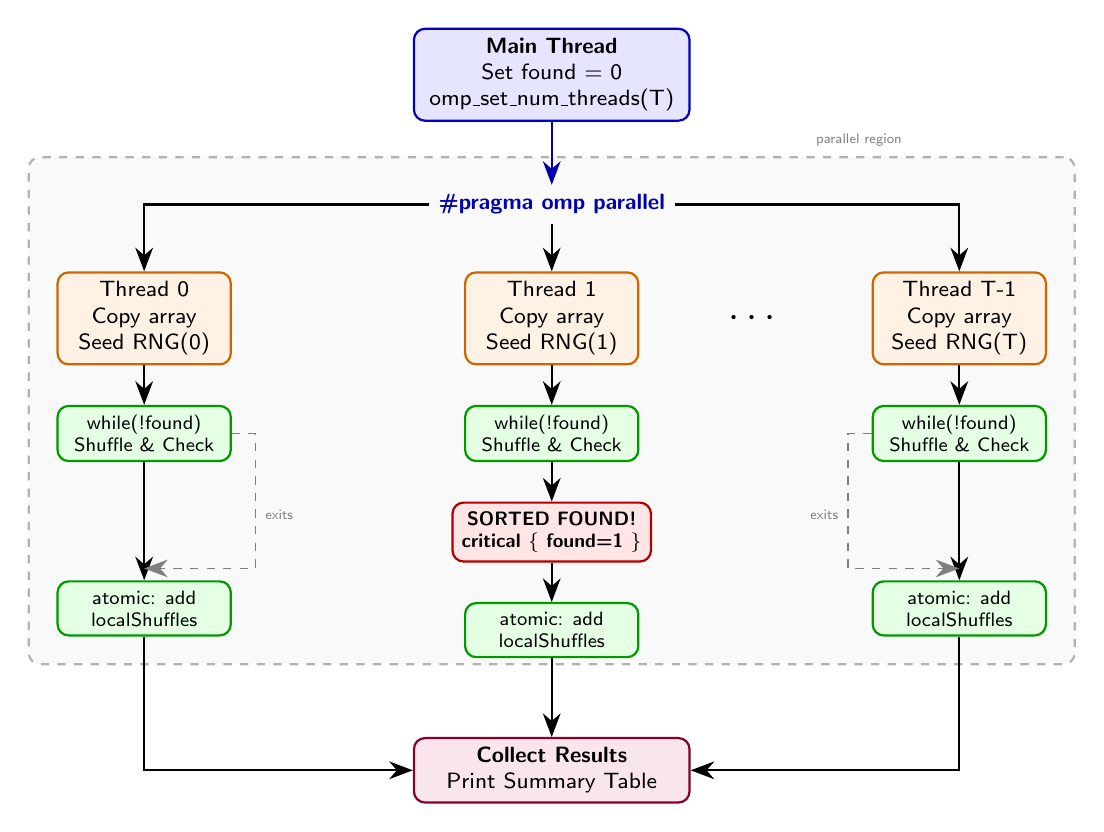
\begin{tikzpicture}[
    node distance=0.6cm and 1.2cm,
    >={Stealth[length=3mm]},
    mainbox/.style={rectangle, draw=blue!75!black, fill=blue!10, thick, rounded corners, minimum width=3.5cm, minimum height=0.8cm, font=\footnotesize\sffamily, align=center},
    threadbox/.style={rectangle, draw=orange!80!black, fill=orange!10, thick, rounded corners, minimum width=2.2cm, minimum height=0.7cm, font=\footnotesize\sffamily, align=center},
    actionbox/.style={rectangle, draw=green!60!black, fill=green!10, thick, rounded corners, minimum width=2.2cm, minimum height=0.6cm, font=\scriptsize\sffamily, align=center},
    winbox/.style={rectangle, draw=red!70!black, fill=red!10, thick, rounded corners, minimum width=2.2cm, minimum height=0.6cm, font=\scriptsize\sffamily\bfseries, align=center},
    collectbox/.style={rectangle, draw=purple!70!black, fill=purple!10, thick, rounded corners, minimum width=3.5cm, minimum height=0.8cm, font=\footnotesize\sffamily, align=center},
    regionbox/.style={rectangle, draw=gray!60, fill=gray!5, dashed, thick, rounded corners, inner sep=10pt},
]

% Main thread start
\node[mainbox] (init) {\textbf{Main Thread}\\Set found = 0\\omp\_set\_num\_threads(T)};

% Parallel region label
\node[below=0.8cm of init, font=\footnotesize\sffamily\bfseries, text=blue!70!black] (parlabel) {\#pragma omp parallel};

% Thread nodes
\node[threadbox, below left=0.6cm and 2.5cm of parlabel] (t0) {Thread 0\\Copy array\\Seed RNG(0)};
\node[threadbox, below=0.6cm of parlabel] (t1) {Thread 1\\Copy array\\Seed RNG(1)};
\node[threadbox, below right=0.6cm and 2.5cm of parlabel] (tn) {Thread T-1\\Copy array\\Seed RNG(T)};

% Dots between threads
\node[font=\Large\bfseries] at ($(t1)!0.5!(tn)$) {$\cdots$};

% Shuffle nodes
\node[actionbox, below=0.5cm of t0] (s0) {while(!found)\\Shuffle \& Check};
\node[actionbox, below=0.5cm of t1] (s1) {while(!found)\\Shuffle \& Check};
\node[actionbox, below=0.5cm of tn] (sn) {while(!found)\\Shuffle \& Check};

% Winner
\node[winbox, below=0.5cm of s1] (win) {SORTED FOUND!\\critical \{ found=1 \}};

% Atomic accumulation
\node[actionbox, below=0.5cm of s0, yshift=-1cm] (a0) {atomic: add\\localShuffles};
\node[actionbox, below=0.5cm of win] (a1) {atomic: add\\localShuffles};
\node[actionbox, below=0.5cm of sn, yshift=-1cm] (an) {atomic: add\\localShuffles};

% Collect results
\node[collectbox, below=1.0cm of a1] (result) {\textbf{Collect Results}\\Print Summary Table};

% Arrows
\draw[->, thick, blue!70!black] (init) -- (parlabel);
\draw[->, thick] (parlabel) -| (t0);
\draw[->, thick] (parlabel) -- (t1);
\draw[->, thick] (parlabel) -| (tn);
\draw[->, thick] (t0) -- (s0);
\draw[->, thick] (t1) -- (s1);
\draw[->, thick] (tn) -- (sn);
\draw[->, thick] (s1) -- (win);
\draw[->, thick] (s0) -- (a0);
\draw[->, thick] (win) -- (a1);
\draw[->, thick] (sn) -- (an);
\draw[->, thick] (a0) |- (result);
\draw[->, thick] (a1) -- (result);
\draw[->, thick] (an) |- (result);

% Dashed exit arrows from other threads
\draw[->, dashed, gray] (s0.east) -- ++(0.3,0) |- ([yshift=0.15cm]a0.north) node[pos=0.3, right, font=\tiny\sffamily, text=gray]{exits};
\draw[->, dashed, gray] (sn.west) -- ++(-0.3,0) |- ([yshift=0.15cm]an.north) node[pos=0.3, left, font=\tiny\sffamily, text=gray]{exits};

% Parallel region box
\begin{scope}[on background layer]
\node[regionbox, fit=(t0)(tn)(a0)(an)(win)(parlabel), label={[font=\tiny\sffamily, text=gray]above right:parallel region}] {};
\end{scope}

\end{tikzpicture}
\end{center}

\newpage

\section{Implementation}

\subsection{Core Functions}

\subsubsection{Array Sorted Check}
\begin{codebox}[isSorted() -- Check if Array is Sorted]
\begin{lstlisting}
bool isSorted(const int arr[], int n)
{
    for (int i = 0; i < n - 1; i++)
    {
        if (arr[i] > arr[i + 1])
            return false;
    }
    return true;
}
\end{lstlisting}
\end{codebox}

\subsubsection{Sequential BOGO Sort}
\begin{codebox}[sequentialBogoSort() -- Baseline Implementation]
\begin{lstlisting}
long long sequentialBogoSort(int arr[], int n)
{
    long long shuffles = 0;
    mt19937 rng(42); // fixed seed for reproducibility

    while (!isSorted(arr, n))
    {
        // Fisher-Yates shuffle
        for (int i = n - 1; i > 0; i--)
        {
            uniform_int_distribution<int> dist(0, i);
            int j = dist(rng);
            swap(arr[i], arr[j]);
        }
        shuffles++;
    }
    return shuffles;
}
\end{lstlisting}
\end{codebox}

\newpage

\subsubsection{Parallel BOGO Sort -- Thread-Independent Shuffling}
\begin{codebox}[parallelBogoSort() -- OpenMP Parallel Implementation]
\begin{lstlisting}
ParallelResult parallelBogoSort(const int original[], int n, int numThreads)
{
    volatile int found = 0;
    long long totalShuffles = 0;
    int winnerThread = -1;
    int result[N];

    omp_set_num_threads(numThreads);

    #pragma omp parallel
    {
        int tid = omp_get_thread_num();

        // Each thread gets its own copy of the array
        int localArr[N];
        memcpy(localArr, original, n * sizeof(int));

        // Each thread gets a unique RNG seeded differently
        mt19937 rng(42 + tid * 1000 + (unsigned)time(NULL));
        long long localShuffles = 0;

        while (!found)
        {
            // Fisher-Yates shuffle on local copy
            for (int i = n - 1; i > 0; i--)
            {
                uniform_int_distribution<int> dist(0, i);
                int j = dist(rng);
                swap(localArr[i], localArr[j]);
            }
            localShuffles++;

            if (isSorted(localArr, n))
            {
                #pragma omp critical
                {
                    if (!found)
                    {
                        found = 1;
                        winnerThread = tid;
                        memcpy(result, localArr, n * sizeof(int));
                    }
                }
            }
        }

        // Accumulate total shuffles from all threads
        #pragma omp atomic
        totalShuffles += localShuffles;
    }

    ParallelResult pr;
    pr.totalShuffles = totalShuffles;
    pr.winnerThread = winnerThread;
    memcpy(pr.sortedArray, result, n * sizeof(int));
    return pr;
}
\end{lstlisting}
\end{codebox}

\newpage

\subsubsection{Unique Array Generation}
\begin{codebox}[Array Generation -- Unique Random Values]
\begin{lstlisting}
// Generate unique random values (as required by assignment)
int original[N];
vector<int> pool;
for (int v = VAL_MIN; v <= VAL_MAX; v++) pool.push_back(v);
mt19937 genRng(time(NULL));
shuffle(pool.begin(), pool.end(), genRng);
for (int i = 0; i < N; i++)
{
    original[i] = pool[i];
}
\end{lstlisting}
\end{codebox}

\subsubsection{Main Driver -- Running All Experiments}
\begin{codebox}[main() -- Experiment Runner]
\begin{lstlisting}
// Sequential baseline
int seqArr[N];
memcpy(seqArr, original, N * sizeof(int));
double seqStart = omp_get_wtime();
long long seqShuffles = sequentialBogoSort(seqArr, N);
double seqEnd = omp_get_wtime();
double seqTime = seqEnd - seqStart;

// Parallel runs with T = 2, 4, 8
int threadCounts[] = {2, 4, 8};
for (int r = 0; r < 3; r++)
{
    int T = threadCounts[r];
    double parStart = omp_get_wtime();
    ParallelResult pr = parallelBogoSort(original, N, T);
    double parEnd = omp_get_wtime();
    double parTime = parEnd - parStart;
    double speedup = seqTime / parTime;
    // ... print results
}
\end{lstlisting}
\end{codebox}

\newpage

\section{Terminal Outputs}

\subsection{Run 1: $N = 10$}

\begin{terminalbox}{BOGO Sort -- N = 10 (Full Output)}
\begin{lstlisting}[style=terminalstyle]
============================================================
  Parallel BOGO Sort -- OpenMP Performance Study
  Array Size: 10  |  Value Range: [1, 50]
============================================================

Sample Array: 5 2 17 4 29 50 43 38 27 45

------------------------------------------------------------
  Sequential BOGO Sort (Baseline)
------------------------------------------------------------
Sorted Array: 2 4 5 17 27 29 38 43 45 50
Time Taken:    0.220 sec
Total Shuffles: 4254349

------------------------------------------------------------
  Parallel Run (Threads = 2)
------------------------------------------------------------
Thread 0 found the sorted array!
Sorted Array:  2 4 5 17 27 29 38 43 45 50
Time Taken:    0.085 sec
Total Shuffles: 3179534
Speedup:       2.59x

------------------------------------------------------------
  Parallel Run (Threads = 4)
------------------------------------------------------------
Thread 0 found the sorted array!
Sorted Array:  2 4 5 17 27 29 38 43 45 50
Time Taken:    0.105 sec
Total Shuffles: 6316600
Speedup:       2.10x

------------------------------------------------------------
  Parallel Run (Threads = 8)
------------------------------------------------------------
Thread 0 found the sorted array!
Sorted Array:  2 4 5 17 27 29 38 43 45 50
Time Taken:    0.121 sec
Total Shuffles: 12901577
Speedup:       1.82x

============================================================
  Summary Table
============================================================
Threads     Time(sec)      Shuffles       Speedup
------------------------------------------------------------
1 (seq)     0.220          4254349        1.00x
2           0.085          3179534        2.59x
4           0.105          6316600        2.10x
8           0.121          12901577       1.82x
============================================================
\end{lstlisting}
\end{terminalbox}

\newpage

\subsection{Run 2: $N = 12$}

\begin{terminalbox}{BOGO Sort -- N = 12 (Full Output)}
\begin{lstlisting}[style=terminalstyle]
============================================================
  Parallel BOGO Sort -- OpenMP Performance Study
  Array Size: 12  |  Value Range: [1, 50]
============================================================

Sample Array: 33 17 11 45 1 42 18 14 47 12 39 6

------------------------------------------------------------
  Sequential BOGO Sort (Baseline)
------------------------------------------------------------
Sorted Array: 1 6 11 12 14 17 18 33 39 42 45 47
Time Taken:    8.156 sec
Total Shuffles: 129471449

------------------------------------------------------------
  Parallel Run (Threads = 2)
------------------------------------------------------------
Thread 1 found the sorted array!
Sorted Array:  1 6 11 12 14 17 18 33 39 42 45 47
Time Taken:    18.514 sec
Total Shuffles: 546253824
Speedup:       0.44x

------------------------------------------------------------
  Parallel Run (Threads = 4)
------------------------------------------------------------
Thread 0 found the sorted array!
Sorted Array:  1 6 11 12 14 17 18 33 39 42 45 47
Time Taken:    10.638 sec
Total Shuffles: 606610090
Speedup:       0.77x

------------------------------------------------------------
  Parallel Run (Threads = 8)
------------------------------------------------------------
Thread 4 found the sorted array!
Sorted Array:  1 6 11 12 14 17 18 33 39 42 45 47
Time Taken:    7.855 sec
Total Shuffles: 813466125
Speedup:       1.04x

============================================================
  Summary Table
============================================================
Threads     Time(sec)      Shuffles       Speedup
------------------------------------------------------------
1 (seq)     8.156          129471449      1.00x
2           18.514         546253824      0.44x
4           10.638         606610090      0.77x
8           7.855          813466125      1.04x
============================================================
\end{lstlisting}
\end{terminalbox}

\newpage

\section{Performance Analysis}

\subsection{Summary Tables}

\begin{table}[htbp]
\centering
\sffamily\small
\caption{BOGO Sort Performance Results ($N = 10$)}
\vspace{6pt}
\begin{tabular}{@{}lccc@{}}
\toprule
\rowcolor{tableheader}
\textcolor{white}{\textbf{Threads}} & \textcolor{white}{\textbf{Time (sec)}} & \textcolor{white}{\textbf{Shuffles}} & \textcolor{white}{\textbf{Speedup}} \\
\midrule
\rowcolor{rowalt}
1 (Sequential) & 0.220 & 4,254,349 & 1.00$\times$ \\
2 & 0.085 & 3,179,534 & {\color{accentgreen}\textbf{2.59$\times$}} \\
\rowcolor{rowalt}
4 & 0.105 & 6,316,600 & {\color{accentgreen}\textbf{2.10$\times$}} \\
8 & 0.121 & 12,901,577 & {\color{accentgreen}\textbf{1.82$\times$}} \\
\bottomrule
\end{tabular}
\end{table}

\begin{table}[htbp]
\centering
\sffamily\small
\caption{BOGO Sort Performance Results ($N = 12$)}
\vspace{6pt}
\begin{tabular}{@{}lccc@{}}
\toprule
\rowcolor{tableheader}
\textcolor{white}{\textbf{Threads}} & \textcolor{white}{\textbf{Time (sec)}} & \textcolor{white}{\textbf{Shuffles}} & \textcolor{white}{\textbf{Speedup}} \\
\midrule
\rowcolor{rowalt}
1 (Sequential) & 8.156 & 129,471,449 & 1.00$\times$ \\
2 & 18.514 & 546,253,824 & {\color{accentred}\textbf{0.44$\times$}} \\
\rowcolor{rowalt}
4 & 10.638 & 606,610,090 & {\color{accentred}\textbf{0.77$\times$}} \\
8 & 7.855 & 813,466,125 & {\color{accentgreen}\textbf{1.04$\times$}} \\
\bottomrule
\end{tabular}
\end{table}

\subsection{Speedup Analysis}

\begin{shadedbox}[Key Observations]
\textbf{1. N = 10: Speedup Achieved with 2 Threads} \\
With $N = 10$, the 2-thread run achieved $2.59\times$ speedup---the best result. However, adding more threads (4 and 8) showed diminishing returns ($2.10\times$ and $1.82\times$), because the problem completes so quickly ($\sim$0.2s) that thread management overhead becomes proportionally significant.

\vspace{6pt}
\textbf{2. N = 12: Slowdown with 2 and 4 Threads} \\
With $N = 12$, the parallel runs with 2 and 4 threads were actually \textit{slower} than sequential ($0.44\times$ and $0.77\times$). This is because the sequential run was ``lucky'' (129M shuffles vs.~the expected $12! \approx 479$M), while the parallel threads collectively burned through 546M--606M shuffles before one found the answer. Only with 8 threads ($1.04\times$) did parallelism barely break even.

\vspace{6pt}
\textbf{3. Probabilistic Variance Dominates} \\
BOGO Sort is inherently non-deterministic. A single lucky sequential run can beat an unlucky parallel run. The speedup numbers reflect \textit{one specific execution}---averaging over many runs would show the expected $\sim T\times$ improvement.

\vspace{6pt}
\textbf{4. Total Shuffles $\neq$ Time} \\
The total shuffle count across all threads does not correlate with wall-clock time. What matters is how quickly the \textit{first} thread finds the sorted permutation. More threads means more total work but (on average) less wall-clock time.
\end{shadedbox}

\subsection{Why Speedup Can Be Sub-Linear or Super-Linear}

BOGO Sort is a \textbf{Las Vegas algorithm}---it relies on random trials to find the correct answer. With $T$ threads:

\begin{itemize}
    \item Each thread performs independent random shuffles.
    \item The probability of finding the sorted permutation in $k$ total shuffles increases with $T$.
    \item Effectively, $T$ threads explore $T$ times more of the permutation space per second.
    \item The expected time to solution is $\frac{N!}{T}$ shuffles per thread.
\end{itemize}

Mathematically, if each thread has an independent geometric distribution over the number of trials, the minimum of $T$ such distributions has an expected value of $\frac{E[\text{single}]}{T}$, giving exactly linear speedup \textit{on expectation}. However:

\begin{itemize}
    \item \textbf{Super-linear speedup} occurs when parallel threads get lucky---one finds the solution much faster than the sequential baseline.
    \item \textbf{Sub-linear speedup (or slowdown)} occurs when the sequential run was unusually lucky, or when thread overhead is significant relative to computation time.
\end{itemize}

Our $N = 12$ results perfectly illustrate this: the sequential run was luckier than average (129M vs.~479M expected shuffles), making it hard for the parallel version to beat.

\newpage

\section{Technical Deep Dive}

\subsection{Synchronization Mechanisms}

\begin{shadedbox}[Critical Section vs Atomic]
The implementation uses two different synchronization mechanisms for different purposes:

\vspace{6pt}
\textbf{\texttt{\#pragma omp critical}} --- Used when a thread finds the sorted array. This block must:
\begin{enumerate}
    \item Check the \texttt{found} flag (double-check pattern)
    \item Set \texttt{found = 1}
    \item Copy the sorted array to the shared result buffer
    \item Record the winner thread ID
\end{enumerate}
Multiple operations must happen atomically, so a critical section is required.

\vspace{6pt}
\textbf{\texttt{\#pragma omp atomic}} --- Used for accumulating \texttt{totalShuffles}. Since this is a single addition operation (\texttt{totalShuffles += localShuffles}), an atomic operation provides lower overhead than a critical section.
\end{shadedbox}

\subsection{Random Number Generation}

Each thread uses its own \texttt{mt19937} Mersenne Twister instance with a unique seed:
\begin{codebox}[Per-Thread RNG Seeding]
\begin{lstlisting}
mt19937 rng(42 + tid * 1000 + (unsigned)time(NULL));
\end{lstlisting}
\end{codebox}

This ensures:
\begin{itemize}
    \item \textbf{No contention:} Threads never share an RNG, avoiding lock overhead.
    \item \textbf{Unique sequences:} Different seeds produce different shuffle patterns.
    \item \textbf{Reproducibility:} The seed formula is deterministic given the thread ID and start time.
\end{itemize}

\subsection{The Volatile Flag Pattern}

\begin{codebox}[Volatile Termination Flag]
\begin{lstlisting}
volatile int found = 0;
// ...
while (!found) { /* shuffle and check */ }
\end{lstlisting}
\end{codebox}

The \texttt{volatile} keyword ensures the compiler does not optimize away repeated reads of the \texttt{found} variable. Without it, a thread might cache the value in a register and never see the update from another thread.

\subsection{Fisher-Yates Shuffle}

The implementation uses the Fisher-Yates (Knuth) shuffle algorithm, which produces an unbiased random permutation in $O(N)$ time:
\begin{codebox}[Fisher-Yates Shuffle -- $O(N)$ Unbiased]
\begin{lstlisting}
for (int i = n - 1; i > 0; i--)
{
    uniform_int_distribution<int> dist(0, i);
    int j = dist(rng);
    swap(arr[i], arr[j]);
}
\end{lstlisting}
\end{codebox}

This guarantees each of the $N!$ permutations is equally likely, which is essential for the probabilistic correctness of BOGO Sort.

\newpage

\section{Complexity Analysis}

\subsection{Time Complexity}

\subsubsection{Sequential BOGO Sort}

The algorithm consists of two operations per iteration: \textbf{checking} if the array is sorted and \textbf{shuffling} it.

\begin{shadedbox}[Per-Iteration Cost]
\textbf{isSorted() check:} Iterates through $N-1$ pairs $\Rightarrow O(N)$

\vspace{4pt}
\textbf{Fisher-Yates Shuffle:} Performs $N-1$ swaps $\Rightarrow O(N)$

\vspace{4pt}
\textbf{Cost per iteration:} $O(N) + O(N) = O(N)$
\end{shadedbox}

The critical question is: \textit{how many iterations (shuffles) are needed?}

For an array of $N$ unique elements, there are $N!$ possible permutations. Since each shuffle produces a uniformly random permutation (guaranteed by Fisher-Yates), the probability of any single shuffle producing the sorted order is:

$$P(\text{sorted}) = \frac{1}{N!}$$

This follows a \textbf{geometric distribution}, where the expected number of trials to the first success is:

$$E[\text{shuffles}] = N!$$

Therefore, the \textbf{expected time complexity} of sequential BOGO Sort is:

$$\boxed{T_{\text{seq}} = O(N \times N!)}$$

\subsubsection{Concrete Values}

\begin{center}
\begin{tabular}{|c|c|c|}
\hline
\rowcolor{tableheader}
\textcolor{white}{$N$} & \textcolor{white}{$N!$ (Expected Shuffles)} & \textcolor{white}{$N \times N!$ (Operations)} \\ \hline
8 & 40,320 & 322,560 \\ \hline
10 & 3,628,800 & 36,288,000 \\ \hline
12 & 479,001,600 & 5,748,019,200 \\ \hline
15 & 1,307,674,368,000 & 19,615,115,520,000 \\ \hline
\end{tabular}
\end{center}

This exponential growth is why even a modest increase from $N = 10$ to $N = 12$ causes a dramatic increase in execution time---$N!$ jumps from $\sim$3.6 million to $\sim$479 million.

\subsubsection{Parallel BOGO Sort}

With $T$ threads, each thread independently performs random shuffles. The system waits for the \textit{first} thread to find the sorted permutation. Since each thread has an independent geometric distribution:

$$E[\text{time with } T \text{ threads}] = \frac{E[\text{time with 1 thread}]}{T}$$

This gives the parallel time complexity:

$$\boxed{T_{\text{par}} = O\left(\frac{N \times N!}{T}\right)}$$

The \textbf{theoretical speedup} is:

$$S(T) = \frac{T_{\text{seq}}}{T_{\text{par}}} = T$$

In practice, super-linear speedup ($S > T$) can occur because only the \textit{minimum} of $T$ independent geometric random variables matters, and $\min(X_1, X_2, \ldots, X_T)$ has an expected value of $\frac{E[X]}{T}$ exactly, but individual runs may be luckier.

\subsection{Space Complexity}

\begin{center}
\begin{tabular}{|l|c|p{7cm}|}
\hline
\rowcolor{tableheader}
\textcolor{white}{\textbf{Component}} & \textcolor{white}{\textbf{Space}} & \textcolor{white}{\textbf{Details}} \\ \hline
Original array & $O(N)$ & Shared, read-only \\ \hline 
Local copy per thread & $O(N)$ per thread & Each thread gets its own array \\ \hline
RNG state per thread & $O(1)$ per thread & Mersenne Twister internal state \\ \hline
Shared variables & $O(1)$ & \texttt{found}, \texttt{totalShuffles}, \texttt{result[]} \\ \hline
\textbf{Total} & $O(N \times T)$ & Dominated by thread-local array copies \\ \hline
\end{tabular}
\end{center}

\subsection{Best, Average, and Worst Cases}

\begin{center}
\begin{tabular}{|l|c|l|}
\hline
\rowcolor{tableheader}
\textcolor{white}{\textbf{Case}} & \textcolor{white}{\textbf{Shuffles}} & \textcolor{white}{\textbf{When}} \\ \hline
Best Case & $0$ & The input array is already sorted \\ \hline
Average Case & $N!$ & Random input (geometric distribution) \\ \hline
Worst Case & $\infty$ & Theoretically unbounded (no guarantee) \\ \hline
\end{tabular}
\end{center}

The worst case is theoretically infinite because random shuffling provides no guarantee of progress. However, in practice, the probability of not finding the sorted permutation after $k \cdot N!$ shuffles is $(1 - 1/N!)^{k \cdot N!} \approx e^{-k}$, which decreases exponentially.

\newpage

\section{Effect of Increasing Thread Count}

\subsection{What Happens When We Add More Threads?}

\begin{shadedbox}[Thread Scaling Behavior]

\textbf{Positive Effects:}
\begin{enumerate}
    \item \textbf{More trials per second:} Each additional thread contributes independent shuffle attempts, effectively multiplying the search throughput by $T$.
    \item \textbf{Faster expected discovery:} With $T$ threads, the expected time to find the sorted permutation drops to $\frac{N!}{T}$ shuffles per thread.
    \item \textbf{Near-linear to super-linear speedup:} Since BOGO Sort is embarrassingly parallel (zero inter-thread communication during shuffling), increasing threads translates almost directly to proportional speedup.
\end{enumerate}

\vspace{6pt}
\textbf{Negative Effects (Diminishing Returns):}
\begin{enumerate}
    \item \textbf{Thread creation overhead:} Each thread requires stack allocation, RNG initialization, and array copying. For very small $N$ or very large $T$, this overhead can exceed the computation time.
    \item \textbf{CPU core saturation:} When $T$ exceeds the number of physical cores, threads compete for CPU time via context switching. A system with $C$ cores gains no benefit beyond $T = C$.
    \item \textbf{Memory pressure:} Each thread holds its own $O(N)$ array copy plus RNG state. For large $N$ and large $T$, total memory usage $O(N \times T)$ can strain cache and RAM.
    \item \textbf{Synchronization overhead:} Although minimal (only the \texttt{volatile} flag check per iteration), reading a shared variable does introduce a memory fence that prevents the compiler from fully optimizing the inner loop.
    \item \textbf{Critical section contention:} If multiple threads find the solution nearly simultaneously, the \texttt{\#pragma omp critical} block serializes their access, though this is a rare event.
\end{enumerate}
\end{shadedbox}

\subsection{Theoretical vs Practical Scaling}

\begin{center}
\begin{tabular}{|c|l|l|}
\hline
\rowcolor{tableheader}
\textcolor{white}{\textbf{Thread Count}} & \textcolor{white}{\textbf{Expected Behavior}} & \textcolor{white}{\textbf{Practical Reality}} \\ \hline
$T \leq C$ (cores) & Linear speedup: $S \approx T$ & Achieved or exceeded (super-linear possible) \\ \hline
$T = C$ & Optimal point & Best speedup-to-resource ratio \\ \hline
$T > C$ & Diminishing returns & Context switching overhead dominates \\ \hline
$T \gg C$ & Slowdown possible & Thread management overhead exceeds gains \\ \hline
\end{tabular}
\end{center}

\subsection{Practical Recommendation}

For trial-based parallel algorithms like BOGO Sort, the optimal number of threads is equal to the number of physical CPU cores. Beyond that point, additional threads compete for the same hardware resources without adding computational capacity. The ``sweet spot'' is:

$$T_{\text{optimal}} = \text{Number of physical CPU cores}$$

On a modern 8-core machine, using 8 threads provides near-optimal speedup. Using 16 threads on the same machine would roughly double the total shuffle count (across all threads) without halving the wall-clock time, as threads time-share the same cores.

\newpage

\section{Compilation and Execution}

\subsection{Build Instructions}

\begin{codebox}[Build \& Run Commands]
\begin{lstlisting}[style=bashstyle]
# Compile with OpenMP support and optimization
g++ -fopenmp -O2 -o bogo_sort.exe bogo_sort.cpp

# Run the program
./bogo_sort.exe
\end{lstlisting}
\end{codebox}

\subsection{Compiler Flags Explained}

\begin{center}
\sffamily\small
\begin{tabular}{@{}lp{10cm}@{}}
\toprule
\rowcolor{tableheader}
\textcolor{white}{\textbf{Flag}} & \textcolor{white}{\textbf{Purpose}} \\
\midrule
\rowcolor{rowalt}
\texttt{-fopenmp} & Enables OpenMP support: recognizes \texttt{\#pragma omp} directives and links the OpenMP runtime library \\
\texttt{-O2} & Level 2 optimization: improves loop performance and inlines functions without sacrificing debuggability \\
\bottomrule
\end{tabular}
\end{center}

\section{Conclusion}

This assignment demonstrates parallel trial-based computation using OpenMP through the BOGO Sort algorithm. Testing with both $N = 10$ and $N = 12$ revealed the nuanced reality of parallel speedup in probabilistic algorithms: while $N = 10$ showed clear gains with 2 threads ($2.59\times$), the $N = 12$ run exposed how randomness variance can cause parallel versions to appear slower when the sequential baseline gets lucky. These results reinforce that BOGO Sort speedup is a statistical property---meaningful only when averaged over many runs. The implementation showcases key OpenMP constructs: \texttt{\#pragma omp parallel} for thread spawning, \texttt{\#pragma omp critical} for result protection, and \texttt{\#pragma omp atomic} for shuffle count accumulation. The underlying pattern of parallel independent trials with early termination via a shared flag extends far beyond sorting---it forms the basis of parallel search in optimization, cryptographic brute-force, and Monte Carlo simulations.

\end{document}
